\documentclass{article}
\usepackage{xcolor}
\usepackage[preprint]{corl_2026}
\usepackage{graphicx,booktabs,amsmath,microtype}
\usepackage[T1]{fontenc}
\graphicspath{{figures/}}
\definecolor{mover}{HTML}{147D92}
\definecolor{reference}{HTML}{C46635}
\title{Same Goal, Different Words:\\Spatial Instruction Sensitivity in World--Action Models}
\author{Anonymous Authors}
\hypersetup{pdftitle={Same Goal, Different Words: Spatial Instruction Sensitivity in World-Action Models},pdfsubject={Draft for Do Robots Need World Models? CoRL 2026 Workshop},pdfauthor={Anonymous Authors}}

\begin{document}
\maketitle
\begin{abstract}
A robot should respond to the requested physical goal, not to one favored way of describing it. We test this requirement by asking three world--action models to perform the same placement while naming either the moved object or the reference object first in the spatial relation. Across 864 matched rollouts on four RoboLab scenes, reference-first descriptions produce fewer stable spatial outcomes, with an average gap of 12.2 percentage points. This gap is concentrated in particular relations rather than shared uniformly across scenes. We also find that reaching a spatial arrangement does not establish that it will be retained or that the intended object was moved. These findings motivate a more discriminating evaluation of world--action models: test alternative descriptions of the same goal, examine individual relations, and distinguish reaching a spatial arrangement from completing the instruction.
\end{abstract}
\keywords{World--Action Models, Spatial Language, Robot Evaluation}

\section{Introduction}
Placing a mustard bottle to the right of a raisin box also leaves the box to the bottle's left. Both descriptions specify the same arrangement, and both instructions can explicitly identify the bottle as the object to move. If behavior changes from the same starting state, physical task difficulty alone cannot explain the difference.

This is a useful test for world--action models, which generate actions alongside predictions of future observations. For robot control, predictive capability should be assessed alongside reliable goal conditioning. We ask: \emph{when the physical goal and initial state stay fixed, does reversing the description of the spatial relation change what the model accomplishes?}

Instruction sensitivity is already established in robot learning. LIBERO-Plus evaluates language perturbations~\citep{fei2026liberoplus}, LIBERO-Para tests meaning-preserving paraphrases from shared starts~\citep{kim2026liberopara}, and semantic guidance for world--action models targets instruction alignment~\citep{he2026sgwam}. We test relational reference inversion across three world--action policies in RoboLab~\citep{yang2026robolab}, using shared starts to control scene difficulty~\citep{li2025simpler}.

\begin{table}[!t]
\caption{One goal, three instructions. Each instruction is tested in a separate run of the same model from the same starting scene. The requested placement and model settings stay fixed.}
\label{tab:setup}
\small
\begin{minipage}[c]{.28\linewidth}
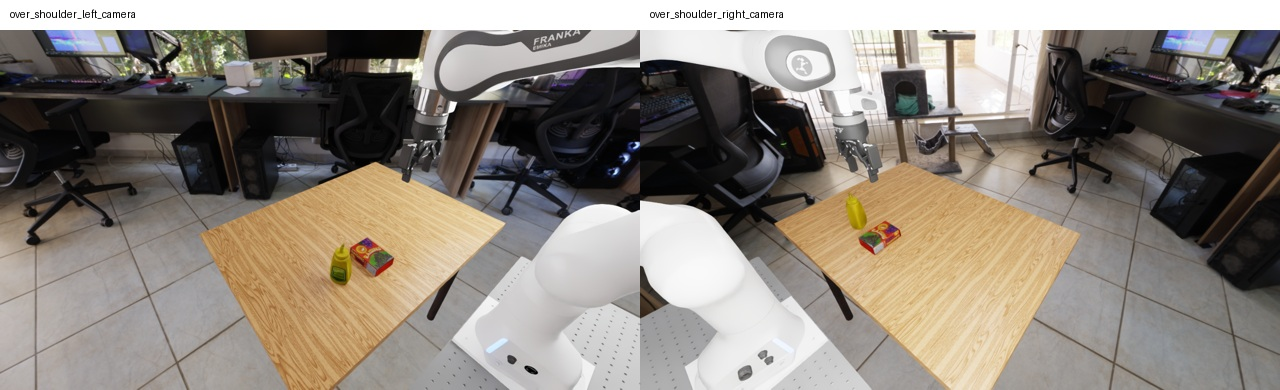
\includegraphics[width=\linewidth]{scene_mustard.jpg}
\end{minipage}\hfill
\begin{minipage}[c]{.68\linewidth}
\textbf{Example goal: mustard to the right of the box.}\par
\textbf{Target:} the mustard bottle, which the robot should move.\par
\textbf{Reference:} the raisin box, which defines the destination.
\end{minipage}\par\medskip
\begin{tabular}{@{}p{.21\linewidth}p{.75\linewidth}@{}}
\toprule
\textbf{Instruction form} & \textbf{Exact tested instruction} \\
\midrule
Direct (D) & Place the mustard bottle on the table to the right of the raisin box. \\
\addlinespace
\textcolor{mover}{Mover-first (S)} & Move the mustard bottle on the table so that \textbf{the mustard bottle} is to the right of the raisin box. \\
\addlinespace
\textcolor{reference}{Reference-first (I)} & Move the mustard bottle on the table so that \textbf{the raisin box} is to the left of the mustard bottle. \\
\midrule
\textbf{S versus I} & Does describing the same placement through the reference object change the outcome? \\
\addlinespace
\textbf{D versus S} & Does expanding the direct instruction change the outcome? \\
\bottomrule
\end{tabular}
\end{table}

\section{Paired spatial evaluation}
\paragraph{Change the description, hold the goal fixed.}
We use four RoboLab scenes: a cube and bowl, butter and a raisin box, mustard and a raisin box, and two bowls. The cube has four directional goals: left, right, front, and behind. Butter and mustard each have left, right, and supported placement on top; the two bowls have both stacking orders. This gives twelve goals. Seven goals come from RoboLab; we add five alternative placements using the same scenes and objects.

Each model runs each goal from each starting configuration under three instructions (Table~\ref{tab:setup}). The \emph{target} is the object to move; the \emph{reference} locates its destination. \emph{Direct} (D) states the placement briefly, using RoboLab wording where available. \emph{Mover-first} (S) names the target first in the spatial clause; \emph{reference-first} (I) names the reference first and reverses the relation. These labels refer to the clause after ``so that'': all three instructions still ask to move the same object.

For supported placement, ``on top of and supported by'' becomes ``underneath and supporting.'' For bowls, the latter does not explicitly require the nesting used by the success check. We show those results separately.

\paragraph{Compare models from the same starts.}
We evaluate the DROID versions of Cosmos3 Nano~\citep{nvidia2026nano}, Cosmos3 Edge~\citep{nvidia2026edge}, and FLUX 3 Action~\citep{bfl2026fluxaction}. Nano and FLUX are chosen for their strong performance on RoboLab's leaderboard, while Edge provides a smaller Cosmos-family comparison~\citep{robolab2026leaderboard}. All receive images from one wrist and two exterior cameras, together with the robot's state. We slightly vary object positions and orientations and retain the first eight starting configurations per scene that a scripted controller can solve. Each model runs every goal and description from these configurations, giving 864 evaluation episodes. Paired runs begin with identical scene states and observations.

Policies execute 32 actions at a time at 15\,Hz, using the same inference seed and fixed settings for each model. Each episode lasts 20--40\,s, depending on the scene, and continues after the first successful placement. Full instructions and evaluation settings accompany the paper.

\paragraph{Separate reaching a placement from completing the task.}
We count a \emph{stable spatial outcome} when, for at least one second, the requested arrangement holds, the target object has the required support and moves slower than 2\,cm/s, and the gripper is no longer touching it. Spatial directions are defined relative to the robot. This outcome can occur at any point in the episode. An additional analysis checks whether it holds during the final second. Neither score verifies which object was moved: moving the reference may also make the relation true.

Our main comparison is mover-first versus reference-first (S$-$I). For each matched pair, we subtract the reference-first outcome (1 if reached, 0 otherwise) from the mover-first outcome. A positive average means more runs reached the arrangement with mover-first wording. We also compare direct with mover-first wording (D$-$S) to test the effect of expanding the instruction. We average within each scene's goals and then equally across scenes and models; the reported gaps are percentage points.

Cube-right, butter-right, and mustard-left already hold in every saved starting scene. Under the at-any-time score, these goals pass with all three instructions and contribute zero to the differences; we show goals requiring a new arrangement separately. Confidence intervals resample starting configurations within each scene, keeping all models, goals, and descriptions paired; sign-flip tests use Holm correction for the two comparisons.

\clearpage
\section{Results}
\paragraph{Reference-first descriptions produce fewer stable outcomes.}
Naming the target first in the spatial relation leads to more stable outcomes than naming the reference first, with an average gap of 12.2 percentage points (95\% interval: 8.6--15.4; adjusted $p<0.001$). The average has the same sign for all three models (Figure~\ref{fig:wording}), while the direct-versus-expanded contrast is smaller and inconclusive. The additional check at the end of each episode gives a similar reference-inversion gap, so the finding is not explained solely by transient placements.

\begin{figure}[!ht]
\centering
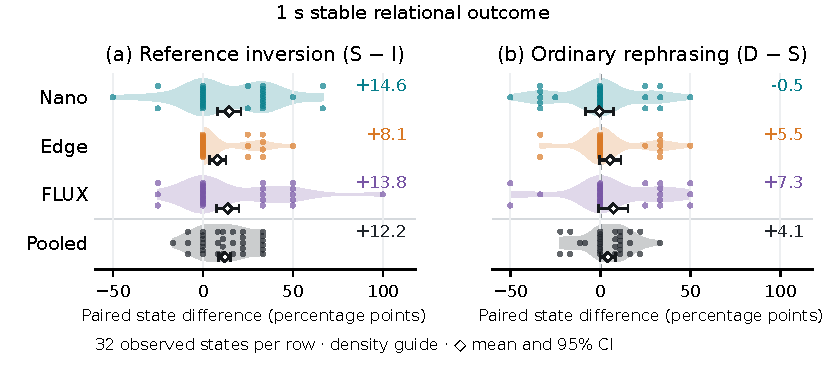
\includegraphics[width=\linewidth]{wording_effect.pdf}
\caption{Paired wording effects. Positive S$-$I favors mover-first descriptions; D$-$S compares direct and expanded wording. Each dot averages paired differences over goals within one start (also over models in the pooled row). Shading guides the eye; diamonds and bars show means and 95\% state-bootstrap intervals. Model-level intervals are descriptive.}
\label{fig:wording}
\end{figure}

\paragraph{A few relations drive the average.}
The largest pooled gap is for mustard-right, with the same direction in all three models. The pooled descriptive gap remains positive when bowl stacking is excluded. In contrast, the cube scene has no aggregate S/I difference, and cube-behind actually favors the reference-first form under the recorded metric. Figure~\ref{fig:goals} exposes these differences: performance varies with the particular scene, relation, and model. This does not establish a general inability to interpret spatial relations.



\paragraph{The success definition changes the interpretation.}
Roughly half of episodes with a stable outcome no longer meet the same conditions at the end. This measures retention under continued control, not performance with success-triggered stopping. Object roles also matter. All seven reference-first cube-behind passes come from Nano episodes with no detected cube lift and substantial bowl displacement. These summaries establish the relation, not that the cube was moved as instructed. A relation score alone cannot distinguish the requested manipulation from movement of the reference.

\clearpage
\begin{figure}[!ht]
\centering
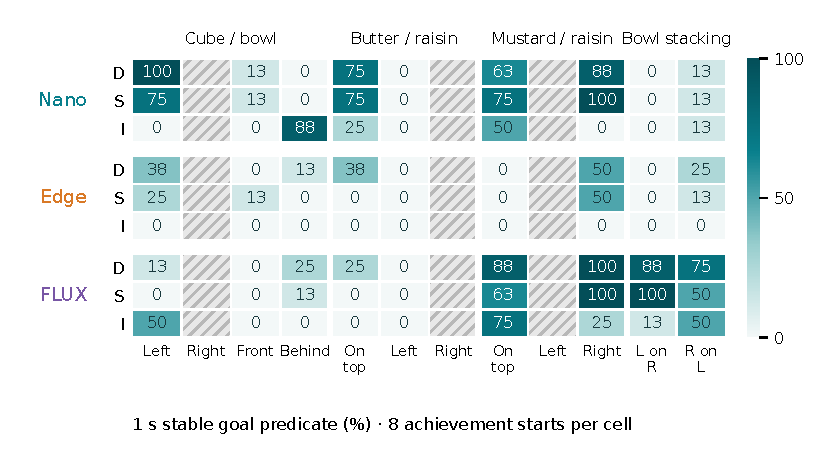
\includegraphics[width=\linewidth]{goal_response_by_form.pdf}
\caption{Reaching a stable spatial arrangement, by goal and wording. Each colored cell has eight starts; hatching marks initially satisfied goals. Relation passes do not verify complete instruction execution, and bowl wording has a support/containment ambiguity.}
\label{fig:goals}
\end{figure}

\section{Discussion}
An instruction specifies both a desired arrangement and an intervention: which object to move to produce it. Equivalent descriptions should preserve these requirements, even when successful trajectories differ. Our paired comparisons show that this consistency cannot be assumed. Shared starts rule out scene difficulty as the sole explanation for the wording gap, but cannot separate a misinterpreted goal from different object selection or execution of an otherwise correct plan.

Mustard-right and cube-behind show why an average is insufficient. Inversion reduces stable outcomes for the former yet improves the relation score for the latter, where passes coincide with substantial bowl displacement. Even a higher score need not establish better instruction following. Evaluation should distinguish whether the requested arrangement was reached, whether the intended manipulation was performed, and whether the arrangement was retained under continued control. These are distinct requirements for reliable behavior.

For world--action models, this raises a question beyond whether predicted futures look plausible: do prediction and action remain consistent with the intended intervention across descriptions? Our behavioral measurements cannot answer it. A useful next test would determine whether wording changes the predicted goal or object motion, and whether execution agrees with that prediction. This requires aligned predictions and executions, with vocabulary and argument order tested separately. Bowl support/containment ambiguity further limits equivalence claims. The aim is to locate failures within instruction following, rather than infer understanding from a relation score alone.

\clearpage
\bibliography{references}
\end{document}
